\documentclass[10pt]{article}
\usepackage{icmlko}

\icmlmeta{IP 파운데이션 월드모델}{307}{손으로 찾은 것을 기계가 다시 찾는다}{노트 306의 결정적 대조를 도구로 만들었다 --- 수선 전 넷을 그대로 짚고 수선 뒤에는 0 이다}

\begin{document}

\twocolumn[
\icmlheader

\begin{abstract}
노트 306이 위키 축의 관측 표시자가 사후라는 것을 \textbf{손으로} 잡았다 ---
계열별 덮음을 세다가 표시자$\sim$라벨 상관이 눈에 띄었고, 코드를 읽어
마스크의 뜻을 알아냈고, ``사전 창 조회수가 둘 다 0 인데 문서 유무만 다른
두 무리''라는 대조를 손으로 만들었다. \textbf{그 대조가 자동화된다.}
\texttt{lab/marker.py} 를 만들었다 --- ① 표시자와 라벨의 상관($|\rho|
{\ge}0.20$, $p{<}0.01$)으로 후보를 고르고 ② \textbf{값이 바닥인 관측 행}과
결측 행의 라벨을 견준다($p{<}0.01$). ②가 열쇠다: 그 축에 대해 \emph{같은
것을 말하는} 두 무리인데 라벨이 갈리면, \textbf{표시자가 값이 안 나르는
무언가를 나른다.} 판 전체에 돌렸다. \textbf{수선 전 --- ``볼 것'' 넷:
게임·위키·유보 · 애니·위키·학습 · 애니·위키·유보 · 웹툰·위키·학습.
노트 306이 손으로 찾은 그 넷이다.} \textbf{수선 뒤 --- 0개.} 그리고 층위가
갈린다: ``바닥만 갈림''으로 남는 셋(모바일·검색·학습 · 웹툰·검색·학습 ·
애니·위키·유보)은 노트 288이 허용한 \emph{정보 있는 결측}이다 --- 검색이
빈 계열을 받은 것은 ``아무도 안 찾았다''는 진짜 측정이라 바닥이 갈리는 것이
당연하다. \textbf{거부권이 아니라 이름표다} --- 표시자가 사후인지는 자료가
어떻게 만들어졌나를 알아야 정해지고 그건 사람이 안다. 도구는 \textbf{어디를
봐야 하는지}를 매 실행에 적는다. \texttt{cfg["표시자"]} 로 붙였다.
\end{abstract}
]

\section{손으로 한 일을 되짚는다}

노트 306의 발견 경로는 이랬다.

\begin{center}\footnotesize
\begin{tabular}{ll}
\hline
① & 계열별 덮음을 세다 표시자$\sim$라벨을 같이 쟀다 \\
② & 위키 셋이 크고 연도 탓이 아닌 것을 봤다 \\
③ & \texttt{wikiaxes} 를 읽어 마스크의 뜻을 알아냈다 \\
④ & \textbf{대조를 만들었다} --- 사전 조회수가 둘 다 0 인 두 무리 \\
\hline
\end{tabular}
\end{center}

①②는 기계가 한다. ③은 사람이 해야 한다. \textbf{④가 자동화된다} ---
그리고 ④가 결론을 낸 자리다.

\section{바닥 대조}

축의 값이 \emph{정보 없음}을 뜻하는 바닥(관측된 것의 하위 10\%)인 행과,
아예 결측인 행은 \textbf{그 축에 대해 같은 것을 말한다.}

\begin{center}\small
\begin{tabular}{ll}
\hline
결측 행 & ``이 축을 모른다'' \\
값이 바닥인 관측 행 & ``이 축이 바닥이다'' \\
\hline
\end{tabular}
\end{center}

둘의 라벨이 갈리면 \textbf{표시자가 값이 안 나르는 무언가를 나른다.}
위키에서 그것이 ``출시 전 조회수 0 인데 문서는 있다'' 대 ``문서가 없다''
였고, 게임 유보에서 7.643 대 9.087($p{=}0.0008$)이었다.

\section{기계가 그 넷을 짚는다}

\begin{figure*}[t]
\centering
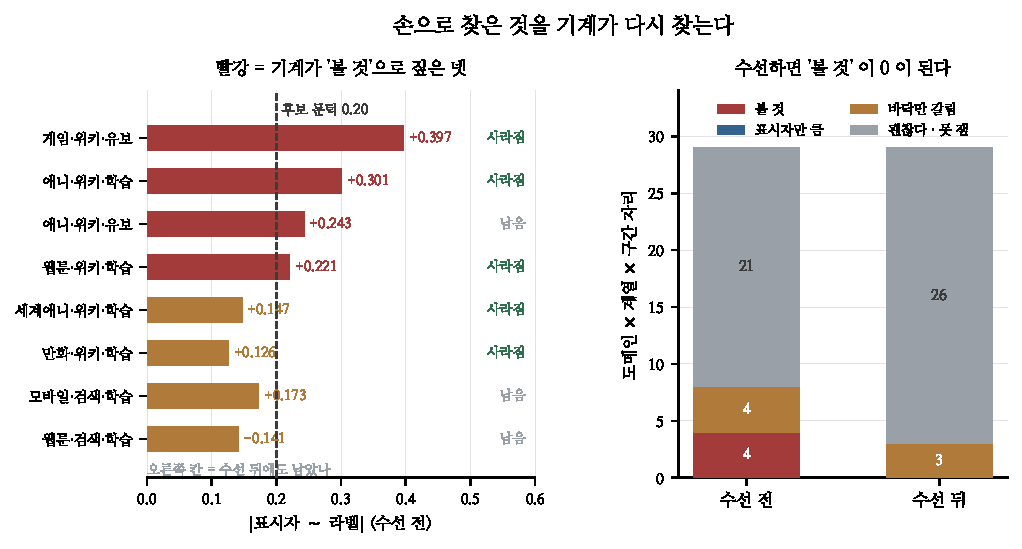
\includegraphics[width=\textwidth]{figs/audit.pdf}
\caption{왼쪽 --- 수선 전 자리별 표시자$\sim$라벨과 판정. 오른쪽 ---
수선 전후의 판정 분포.}
\end{figure*}

\begin{center}\footnotesize
\begin{tabular}{lrrl}
\hline
자리 & $\rho$ & 바닥 $p$ & 판정 \\
\hline
\textbf{게임·위키·유보} & 0.397 & 0.0008 & \textbf{볼 것} \\
\textbf{애니·위키·학습} & 0.301 & $<$1e-4 & \textbf{볼 것} \\
\textbf{애니·위키·유보} & 0.243 & $<$1e-4 & \textbf{볼 것} \\
\textbf{웹툰·위키·학습} & 0.221 & $<$1e-4 & \textbf{볼 것} \\
\hline
모바일·검색·학습 & 0.173 & $<$1e-4 & 바닥만 갈림 \\
세계애니·위키·학습 & 0.147 & 0.0008 & 바닥만 갈림 \\
웹툰·검색·학습 & $-$0.141 & $<$1e-4 & 바닥만 갈림 \\
만화·위키·학습 & 0.126 & $<$1e-4 & 바닥만 갈림 \\
\hline
\end{tabular}
\end{center}

\textbf{``볼 것'' 넷이 노트 306이 손으로 찾은 그 넷이다.} 그리고 수선
(\texttt{zero\_is\_data=False}) 뒤에 다시 돌리면

\begin{center}\small
\begin{tabular}{lrr}
\hline
판정 & 수선 전 & \textbf{수선 뒤} \\
\hline
\textbf{볼 것} & \textbf{4} & \textbf{0} \\
바닥만 갈림 & 4 & 3 \\
괜찮다 · 못 잼 & 21 & 26 \\
\hline
\end{tabular}
\end{center}

\section{층위가 갈리는 것이 중요하다}

``바닥만 갈림''으로 남는 셋은 \textbf{남아야 한다.}

\begin{center}\footnotesize
\begin{tabular}{ll}
\hline
자리 & 왜 괜찮은가 \\
\hline
모바일·검색·학습 & 물어보고 빈 계열을 받았다 --- \\
웹툰·검색·학습 & \quad ``아무도 안 찾았다''는 \textbf{진짜 측정} \\
애니·위키·유보 & 수선 뒤 $\rho$ 0.243$\to$0.098 로 준 잔여 \\
\hline
\end{tabular}
\end{center}

노트 288이 \emph{정보 있는 결측}(게임 \texttt{media\_push} $+$0.405)을
허용한 것과 같은 자리다. \textbf{바닥이 갈린다는 것만으로는 잘못이 아니다}
--- 표시자가 큰 정보를 나르는데 \emph{그 정보의 출처가 사후}일 때만 잘못이다.
그래서 두 검사를 \textbf{둘 다} 통과해야 ``볼 것''이 된다.

\paragraph{그리고 이것이 이름표인 이유} 표시자가 사후인지는 \textbf{자료가
어떻게 만들어졌나}를 알아야 정해진다. 위키는 문서가 없으면 물어볼 대상이
없고, 검색은 물어보고 빈 답을 받는다 --- 같은 ``마스크 0''인데 뜻이 다르다.
\textbf{코드는 그 차이를 모른다.} 그래서 승격을 안 막고
(\texttt{hearing} · \texttt{overlap} 과 같은 규약) 매 실행에 한 줄을 남긴다.

\section{도구 셋이 붙었다}

\begin{center}\footnotesize
\begin{tabular}{lll}
\hline
이름표 & 묻는 것 & 노트 \\
\hline
청력 & 전용 축을 들을 수 있나 & 276$\sim$281 \\
겹침 & 이 축이 새로운가 & 299 · 300 \\
\textbf{표시자} & \textbf{표시자가 값 너머를 나르나} & \textbf{306 · 307} \\
\hline
\end{tabular}
\end{center}

셋 다 \textbf{판정치 옆에 적을 뿐 승격을 안 막는다.} 그리고 셋 다
\textbf{그 이름으로 무엇을 할지는 따로 재야 한다} --- 노트 305가 겹침에서
배운 것이다(세 판정 중 어느 것도 제거의 근거가 아니었다).

\paragraph{남은 것}
\begin{center}\small
\begin{tabular}{ll}
\hline
갈래 & 왜 \\
\hline
표시자를 다른 판에도 & \texttt{wide*} · \texttt{mkt} 축 세트 \\
게임 위키 0.31 & 수선 뒤에도 큰 잔여 \\
바닥 정의를 흔들어 & 하위 10\% 가 임의다 \\
피처 위약 & 노트 302의 갈래 --- 돌고 있다 \\
\hline
\end{tabular}
\end{center}

\paragraph{규약} \textbf{손으로 한 대조는 도구로 만들어라.} 노트 306의
결론을 낸 것은 상관이 아니라 \textbf{대조}였다 --- 상관만 봤으면
``$+$0.397 은 크다'' 에서 멈췄을 것이고, 그것은 ``게임 위키는 좋은 축이다''로
읽힐 수도 있었다. 대조가 ``출시 전 관심이 같은데 갈린다''를 보여 준 뒤에야
사후라고 말할 수 있었다. \textbf{그 한 걸음이 자동화되면 다음번에는
눈에 안 띄어도 잡힌다.}

\end{document}
